\label{cap:resultados}
Este capítulo apresenta os resultados da reconstrução retrospectiva da migração da BSN do ROS 1 para o ROS 2, organizados segundo as atividades da metodologia proposta. São examinadas as evidências de compreensão do sistema legado, a recuperação das especificações comportamentais, a identificação das responsabilidades associadas aos comportamentos selecionados, a caracterização das transformações de migração e a comparação das evidências comportamentais disponíveis nas duas implementações.

\section{Compreensão de Programas na BSN}
\label{sec:compreensao-res}

O processo de compreensão anteriormente aplicado à BSN por Couto~\cite{tgsamuelcouto} fornece uma aplicação concreta desses princípios. A investigação adotou aspectos de uma estratégia \textit{top-down}, partindo do conhecimento prévio sobre o propósito geral da BSN por meio de artigos e examinando progressivamente regiões mais específicas de sua implementação, para com o propósito de formular e verificar hipóteses sobre seu funcionamento. Embora Couto não descreva explicitamente esse procedimento como uma instanciação do \textit{Integrated Metamodel}, o processo também transita entre o conhecimento sobre o sistema em nível mais alto e as evidências no nível da implementação.

Para apoiar essa investigação, Couto construiu visões estáticas e dinâmicas complementares da BSN. A visão estática expõe relações de implementação, como hierarquias de classes, composições, implementações de interfaces, chamadas de métodos e dependências. Na BSN, essa visão foi obtida a partir do código-fonte utilizando Doxygen e sua integração com GraphViz~\cite{tgsamuelcouto}. 

Sob essa perspectiva, podemos verificar o funcionamento de alguns dos principais componentes da BSN ligados ao módulo de \textit{target system}. A figura \ref{fig:sensor} demonstra um exemplo do GraphViz do componente Sensor. Ela guia o entendimento dos principais componentes a partir de chamadas, onde por exemplo, nessa imagem a execução principal da instância de um sensor, ao iniciar a execução com \texttt{run}, chama uma série de métodos do sistema onde podemos ver supor interações ligadas a comunicação à parte adaptativa do sistema como \textit{sendEnergyStatus}, \textit{sendStatus, sendEvent}, o tratamento de energia, \textit{recharge, generate} e o pipeline que envia os dados para o Bodyhub, \textit{collect, process, transfer}.

\begin{figure}[H]
    \centering
    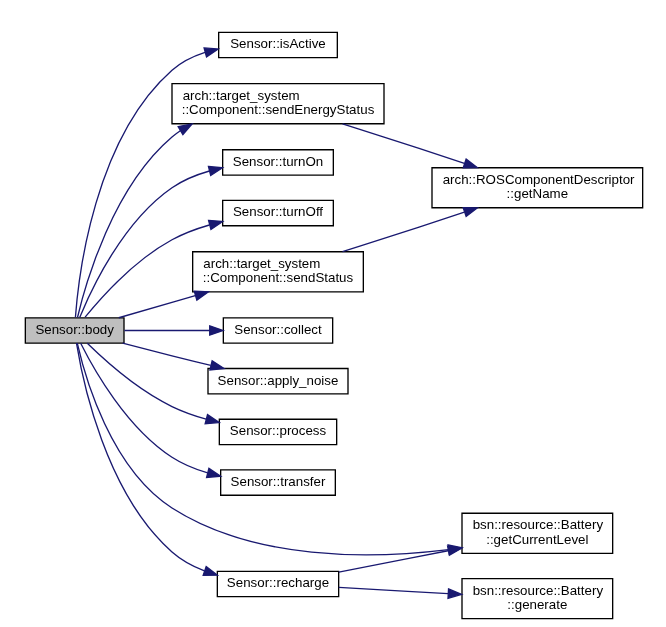
\includegraphics[width=0.7\textwidth]{img/sensorBSN.png}
    \caption{call graph do sensor}
    \label{fig:sensor}
\end{figure}

também podemos verificar o call graph do CentralHub na figura \ref{fig:bodyhub} onde é possível observar chamadas de método similares ao sensores por herdarem de classes comuns, a execução do pipeline que coleta os dados do sensores por callback \textit{collect}, o pipeline do \textit{body} ligado ao gerenciamento de bateria, processamento de dados e transferência para o repositório de conhecimento.

\begin{figure}[H]
    \centering
    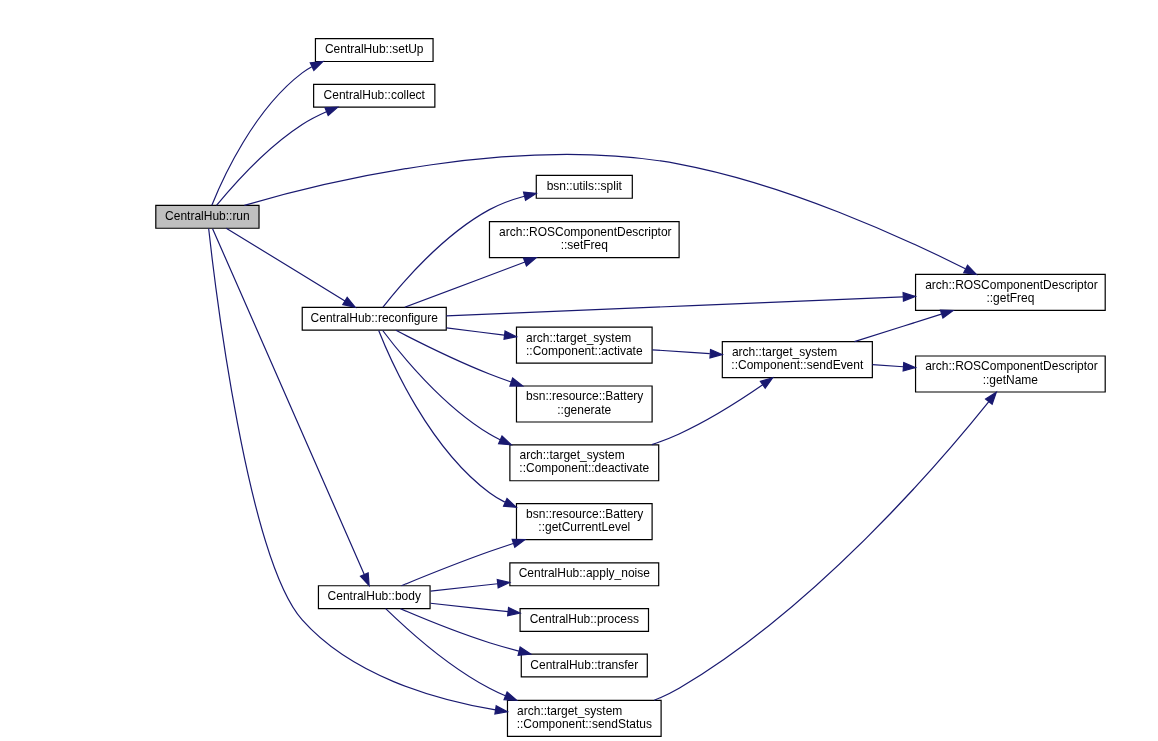
\includegraphics[width=1\textwidth]{img/centralhubrun.png}
    \caption{ call graph do CentralHub}
    \label{fig:bodyhub}
\end{figure}

A visão dinâmica complementa essas informações estruturais ao expor a topologia de comunicação do sistema em execução. Couto utilizou \texttt{rqt\_graph} para visualizar os nós ROS ativos durante a execução, os tópicos publicados e assinados e as relações de comunicação estabelecidas entre eles~\cite{tgsamuelcouto}. 

Essa visão fornece evidências de execução que não são diretamente observáveis na estrutura estática do código-fonte. Nessa visão, podemos observar nós que encaixam na descrição arquitetural da figura \ref{fig:arquitetura} conectado por fluxo de dados chamado de \textit{tópicos}. Componentes caracterizado como /g3t\_n significam sensores enquanto /g4t1 significa CentralHub. Essa nomeclatura foi escolhida devido a abordagem do sistema orientado a \textit{Goal Model }. Para outros módulos, podemos observar o injetor de incertezas pelo /injector,a simulação pelo /patient a partir de serviços,  o a ponte para a adaptação pelo /logger e /collector, o repositório de conhecimento sendo representado pelo /data\_access e o sistema gerenciador relacionado pelo /enactor e /reli\_engine.

\begin{figure}[H]
    \centering
    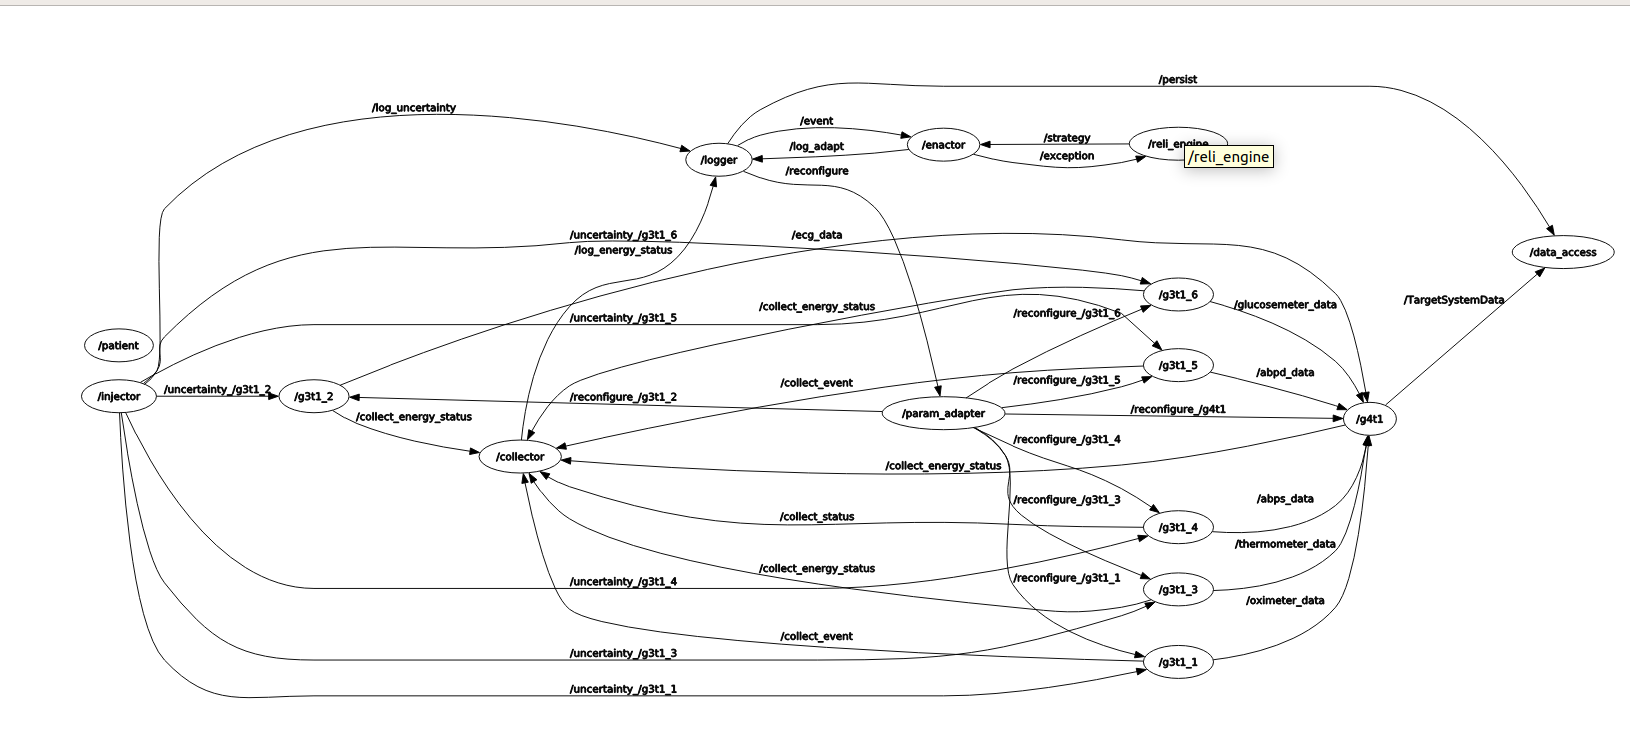
\includegraphics[width=1\textwidth]{img/rqtgraph.png}
    \caption{visão dinâmica da BSN}
    \label{fig:graviz}
\end{figure}

Em suma, a visão estática contribui com evidências sobre a estrutura de implementação e suas dependências, enquanto a visão dinâmica contribui com evidências sobre a comunicação entre nós ROS em tempo de execução. Essas observações são interpretadas em conjunto com a documentação existente e o conhecimento do domínio para melhorar a compreensão do sistema legado do \textit{recoverer}. Esse conhecimento é levado adiante para a Especificação Comportamental, na qual ajuda a mapear propriedades existentes no contexto da BSN em execução, e permanece disponível durante a Identificação das Realizações Comportamentais, na qual evidências de implementação específicas dos cenários são posteriormente interpretadas em termos de componentes e responsabilidades do sistema.

\section{Especificação Comportamental na BSN}
\label{sec:resultados-especificacao-bsn}

A  Especificação Comportamental da BSN foi reconstruída a partir das propriedades do sistema descritas por Rodrigues et al.~\cite{Rodrigues_2018} dos cenários BDD disponíveis para a implementação legada em ROS~1 do aprimoramento e da documentação de sua organização e rastreabilidade no repositório de BSN\_TRACES~\cite{Viana}. O objetivo desta análise é identificar os comportamentos selecionados e apresentar como suas expectativas foram expressas em cenários Gherkin. A análise considera os artefatos do repositório \texttt{richardjlv/bsn\_} \cite{BSN_ROS1_BDD}. 

\paragraph{Origem e delimitação dos comportamentos:}

As propriedades formuladas por Rodrigues et al.~\cite{Rodrigues_2018} constituem uma das principais fontes para especificar expectativas funcionais e temporais da BSN. Sua utilização exige selecionar o aspecto pertinente à aplicação legada, pois a representação original foi elaborada para um modelo e um contexto de verificação específicos. A Tabela~\ref{tab:features-definicoes} apresenta correspondências documentadas entre essas propriedades e cenários disponíveis no ROS~1. Além das propriedades de origem, a especificação inclui critérios complementares associados a interações observáveis entre componentes.




\begin{table}[htbp]
\centering
\caption{Relação entre as propriedades comportamentais da BSN e os cenários BDD do ROS 1}
\label{tab:features-definicoes}

\begin{tabularx}{\textwidth}{@{}
  >{\raggedright\arraybackslash}X
  >{\raggedright\arraybackslash}X@{}}
\toprule
\textbf{Propriedade de origem} &
\textbf{Correspondência com a especificação BDD} \\
\midrule

P3 --- detecção de emergência com limite inclusivo de
250 ms ($\leq 250$ ms) e condição relativa ao ciclo do escalonador &
Base para BSN-P03. O cenário especifica a detecção de emergência
após uma leitura de alto risco, respeitando o limite de 250 ms.
Inclui uma variante sob carga elevada. \\

P8 --- coleta no sensor seguida de persistência eventual no BodyHub &
Base para BSN-P08. Os cenários especificam a persistência
das leituras coletadas, considerando situações nominais
e de falha de armazenamento. \\

P9 --- envio pelo sensor seguido de processamento nas categorias
baixa, moderada ou alta &
Antecedente de BSN-P09. O cenário de classificação de alto
risco representa um recorte dessa propriedade, embora
conserve o identificador histórico P08 em seu título. \\

P10 --- processamento no BodyHub seguido de detecção eventual
de um novo estado de saúde &
Base para BSN-P10. Os cenários especificam a disponibilização
do estado de saúde do paciente e uma variante na qual
o CentralHub está indisponível. \\

P4--P6 --- ajuste da aquisição conforme a categoria de risco &
Antecedentes conceituais da adaptação da aquisição, sem
correspondência direta com os cenários BDD relativos
à adaptação por confiabilidade dos sensores. \\

\bottomrule
\end{tabularx}

\par\smallskip
{\footnotesize
mapeamento das propriedade de \cite{Rodrigues_2018}.
}

\end{table}

\paragraph{Cenários BDD recuperados.}

O levantamento apresentado no repositório~\cite{Viana} organiza a suíte em oito famílias de arquivos \texttt{.feature} e cataloga 24 definições de cenários, identificadas documentalmente como \texttt{BDD01}--\texttt{BDD24} e quinze critérios complementares, \texttt{BSN-C01}--\texttt{BSN-C15}.

O requisito temporal de emergência está representado no arquivo \texttt{BSN-\allowbreak P03.feature}. O arquivo \texttt{check\_\allowbreak bsn.feature} reúne cenários de recepção e classificação de leituras, o \texttt{data\_\allowbreak persistance.feature} aborda persistência e \texttt{health\_\allowbreak status.feature} especifica o estado de saúde do paciente. Outros arquivos \texttt{.feature} registram contratos de monitoramento, adaptação e comunicação. Em conjunto, esses artefatos documentam expectativas comportamentais para a BSN legada.

\paragraph{Exemplo de requisito temporal: detecção de emergência.}

A Listagem~\ref{lst:bsn-p03-ros1} reproduz um cenário da especificação \texttt{BSN-P03.feature}, identificado como \texttt{BDD01} na catalogação. O cenário parte da condição de monitoramento pelo termômetro, considera como estímulo uma leitura na faixa de alto risco e estabelece como resultado esperado a comunicação da emergência pelo CentralHub dentro de 250~ms. Desse modo, o requisito temporal é expressado como uma obrigação observável, sem prescrever quais métodos internos devem executá-la.

\begin{lstlisting}[
    language=Gherkin,
    basicstyle=\small\ttfamily,
    breaklines=true,
    columns=fullflexible,
    caption={Cenário BDD de detecção de emergência (BDD01/BSN-P03).},
    label={lst:bsn-p03-ros1}
]
Scenario: An emergency is reported within 250 ms of a high-risk reading (BSN-P03)
    Given the patient is being monitored by the thermometer
    When the thermometer reports a vital sign reading in the high-risk range
    Then the central hub should report an emergency within 250 ms of that reading
\end{lstlisting}

\paragraph{Exemplo de contrato entre componentes}

Além de propriedades associadas ao comportamento global, os cenários da BSN contemplam interações entre componentes. A Listagem~\ref{lst:bsn-c01-ros1} apresenta o cenário parametrizado \texttt{BDD03}, disponível em \texttt{check\_bsn.feature}. Seu critério de aceitação estabelece que o CentralHub receba a leitura com o valor informado pelo sensor. 

\begin{lstlisting}[
    language=Gherkin,
    basicstyle=\small\ttfamily,
    breaklines=true,
    columns=fullflexible,
    caption={Cenário BDD de recepção de leituras (BDD03/BSN-C01).},
    label={lst:bsn-c01-ros1}
]
Scenario Outline: The central hub receives the vital sign reading reported by a body sensor (BSN-P08)
    Given the patient is being monitored by <sensor>
    When <sensor> reports a new vital sign reading
    Then the central hub should receive that reading with the value reported by <sensor>

    Examples:
        | sensor          |
        | the oximeter    |
        | the ECG sensor  |
        | the thermometer |
        | the SBP sensor  |
        | the DBP sensor  |
        | the glucometer  |
\end{lstlisting}

Nesse exemplo, a variável é identificada por seu papel no domínio (\textit{sensor}) e o comportamento esperado é a correspondência entre a leitura reportada e o valor recebido pelo CentralHub. Esse tipo de cenário ilustra a possibilidade, prevista na metodologia, de formular critérios comportamentais pertinentes às responsabilidades de componentes do sistema.

\paragraph{Síntese dos resultados da etapa.}

No recorte da BSN legada, os produtos identificáveis da Especificação Comportamental são os cenários Gherkin e a correspondência documental entre os critérios de aceitação, suas fontes e os identificadores da suíte. Os exemplos apresentados mostram a tradução de uma propriedade temporal em um cenário BDD e a explicitação de um contrato de recepção entre componentes.

\section{Resultados da Identificação das Realizações dos Comportamentos}
\label{sec:resultados-identificacao-realizacoes}

A aplicação desta etapa teve como objetivo a delimitação das responsabilidades da BSN relevantes à mudança do contexto ROS~1 para ROS~2. A investigação combinou (i)~cenários BDD preservados na implementação legada, (ii)~relações de comunicação e entidades identificadas no código C++, e (iii)~relatórios de cobertura de oito campanhas executadas disponibilizado no repositório \texttt{bsn\_traces}\footnote{\url{https://github.com/richardjlv/bsn_traces/blob/main/INDICE_FEATURES_ROS1.md}}. O resultado consistiu em uma relação entre comportamentos, entidades de implementação e responsabilidades, seguido da delimitação das responsabilidades relevantes para o planejamento das transformações de migração. A sistematização desse material é retrospectiva não replica fielmente as técnicas de \textit{FeatureTrace} ou de \textit{Software Reconnaissance} durante a migração original.

\subsection{Comportamentos e interfaces selecionadas}
\label{subsec:res-identificacao-contratos}

Foram examinados cenários BDD relacionados a transmissão de dados dos sensores, propagação de risco, indisponibilidade do CentralHub e
 infraestrutura de monitoramento e adaptação. A Tabela~\ref{tab:res-identificacao-bdd} sintetiza o recorte utilizado. 

\begin{table}[htbp]
\centering
\caption{Cenários BDD utilizados para localizar e delimitar responsabilidades na BSN}
\label{tab:res-identificacao-bdd}
\scriptsize
\begin{tabularx}{\linewidth}{@{}p{0.17\linewidth}p{0.39\linewidth}X@{}}
\toprule
\textbf{ID} & \textbf{Observação definida no cenário} & \textbf{Interfaces ou elementos de interesse} \\
\midrule
BDD03 / BSN-C01 & A leitura informada pelo sensor deve ser recebida pelo CentralHub com o valor correspondente. & Tópicos de dados dos sensores e \texttt{/TargetSystemData}; sensor e CentralHub. \\
BDD04 / BSN-P09 & Uma leitura de oxigenação em faixa de alto risco deve resultar em risco alto observável na saída do CentralHub. & Avaliação e rótulo do risco no sensor; campos de risco na saída do CentralHub. \\
BDD05 / BSN-C02 & Não deve ser publicado novo risco para a leitura quando o CentralHub estiver indisponível. & Presença operacional do nó \texttt{/g4t1} e publicação da saída. \\
BDD15 / BSN-C07 & O registro do sistema deve receber os tópicos encaminhados pelo coletor de eventos, estados e energia. & \texttt{collect\_*}, \texttt{log\_*}; \textit{probe}/coletor e \textit{logger}. \\
BDD17--18 / BSN-C08--C09 e BDD23 / BSN-C14 & O sistema deve emitir comandos de adaptação e manter a comunicação do adaptador com seus destinatários. & Comandos \texttt{freq}, adaptador de parâmetros e subscrição de reconfiguração. \\
\bottomrule
\end{tabularx}
\end{table}

O cenário BDD03 foi selecionado para exemplificar a identificação das entidades envolvidas na transmissão de dados entre o Sensor e o CentralHub. A identificação das interfaces foi auxiliada pela inspeção das definições de passos do cenário, que utilizam os tópicos do sensor e do \textit{target-system} para observar o comportamento especificado.

\subsection{Localização das realizações no ROS~1}
\label{subsec:res-identificacao-localizacao}

A inspeção de \texttt{Sensor.cpp}, \texttt{G3T1\_3.cpp}, \texttt{CentralHub.cpp} e \texttt{G4T1.cpp} permitiu reconstruir o caminho de BDD03 para a instância do termômetro. Podemos verificar esse caminho no sensor pela figura \ref{fig:sensor}. O método \texttt{Sensor::body()} coordena a coleta, o processamento e a transferência, o \path{G3T1_3::collect()} consulta o simulador do paciente por serviço ROS, \path{G3T1_3::process()} trata a leitura e \path{G3T1_3::transfer()} publica o resultado em \texttt{/thermometer\_data}. A classe \texttt{CentralHub} na figura \ref{fig:bodyhub} susbcreve nesse tópico com o\texttt{G4T1::collect()} recebendo os dados. O processamento posterior de \texttt{G4T1} publica o estado agregado pelo tópico \texttt{/TargetSystemData}. A Figura~\ref{fig:res-bdd03-sequencia} apresenta a relação entre componentes e métodos identificada pela leitura do código e pelas interfaces observadas nos testes. 

\begin{figure}[htbp]
\centering
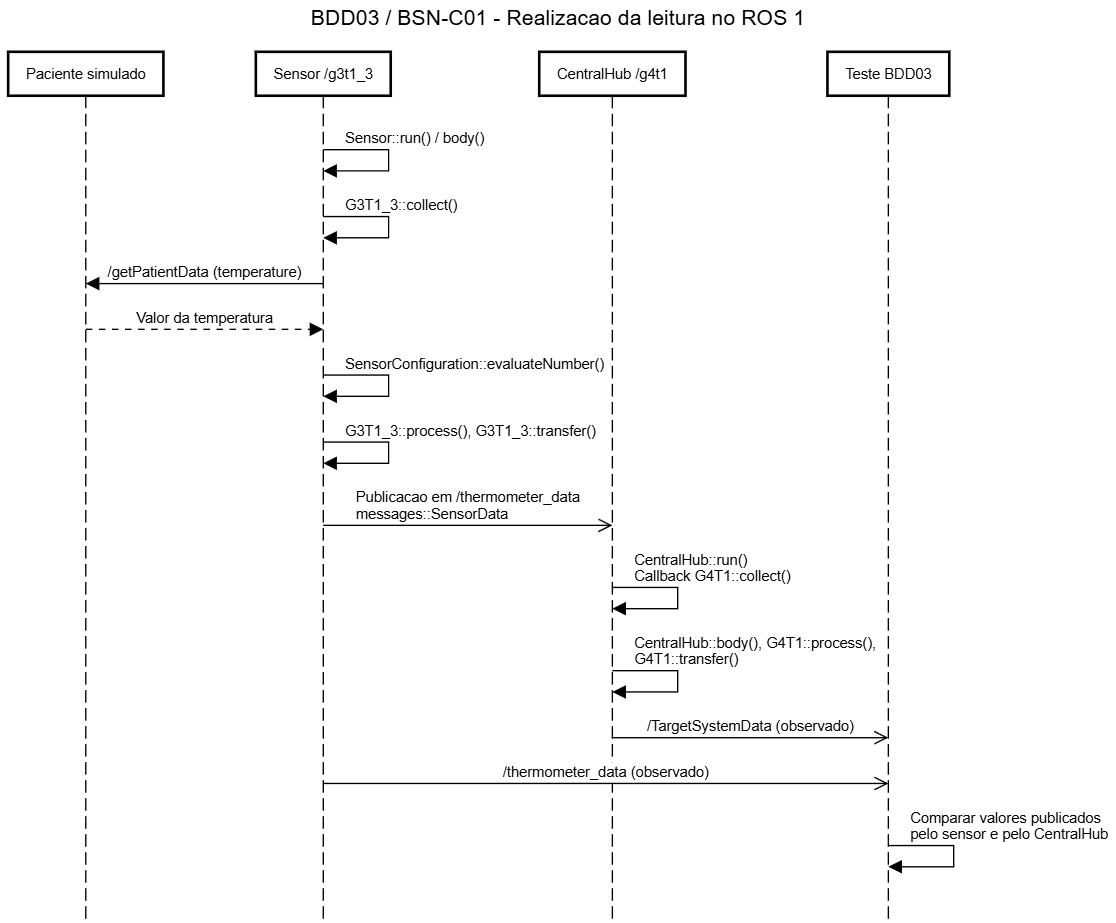
\includegraphics[width=0.97\linewidth]{img/feature ROS1.png}
\caption{Mapeamento estrutural da realização de BDD03/BSN-C01 no ROS~1.
A sequência deriva da inspeção das interfaces e do código; não representa
um rastro individual de chamadas de métodos C++.}
\label{fig:res-bdd03-sequencia}
\end{figure}


A identificação das interfaces de comunicação também foi apoiada pela visão dinâmica da BSN, apresentada na Figura~\ref{fig:graviz}. O grafo permite visualizar os nós ROS e suas relações de publicação e subscrição, fornecendo uma referência para o mapeamento entre os componentes do sistema.

Além da realização detalhada para BDD03, a inspeção da implementação permitiu identificar entidades associadas a outros cenários selecionados. A Tabela~\ref{tab:res-mapeamento-bdd} sintetiza essas associações, que constituem um recorte do \textit{Scenario Realization Mapping}.

\begin{table}[htbp]
\centering
\caption{Mapeamento entre cenários  BDD e
entidades da implementação ROS~1}
\label{tab:res-mapeamento-bdd}
\scriptsize
\begin{tabularx}{\linewidth}
{@{}p{0.19\linewidth}X p{0.31\linewidth}@{}}
\toprule
\textbf{Contrato} &
\textbf{Entidades identificadas} &
\textbf{Responsabilidade} \\
\midrule

BDD03 / BSN-C01 &
\texttt{Sensor::body()},
\texttt{G3T1\_3::transfer()},
\texttt{G4T1::collect()} &
Transmissão e recepção de leituras \\

BDD04 / BSN-P09 &
\texttt{SensorConfiguration::evaluateNumber()},
\texttt{G3T1\_3::transfer()} &
Avaliação e propagação do risco \\

BDD05 / BSN-C02 &
\texttt{CentralHub::run()},
\texttt{CentralHub::body()} &
Disponibilidade e processamento do CentralHub \\

BDD15 / BSN-C07 &
\texttt{Probe},
\texttt{Logger} &
Coleta e encaminhamento de eventos,
estados e informações de energia \\

BDD17--18 / BSN-C08--C09 &
\texttt{Controller},
\texttt{ParamAdapter},
\texttt{Sensor::reconfigure()} &
Adaptação da frequência dos sensores \\

BDD23 / BSN-C14 &
\texttt{ParamAdapter},
\texttt{Sensor::reconfigure()},
\texttt{CentralHub::reconfigure()} &
Encaminhamento e recepção de comandos
de reconfiguração \\

\bottomrule
\end{tabularx}
\end{table}

\subsection{Participação dos métodos nos grupos de testes BDD}
\label{subsec:res-identificacao-caracterizacao}

Os relatórios HTML de cobertura LLVM preservam contagens de execução por linha de código. Para os cinco arquivos examinados (\path{Component.cpp}, \path{Sensor.cpp}, \path{G3T1_3.cpp}, \path{CentralHub.cpp} e \path{G4T1.cpp}), foram verificadas as linhas de entrada de onze métodos selecionados. Considerou-se que um método participou de uma campanha quando a linha correspondente apresentou contagem de execução. Cada campanha corresponde à execução isolada de uma família de cenários BDD, como \texttt{check\_bsn}, relacionada à transmissão de leituras e à classificação de risco, \texttt{health\_status}, à disponibilização do estado de saúde do paciente, e \texttt{managing\_system}, ao monitoramento e à adaptação do sistema. A identificação dos métodos exercitados foi realizada mediante a inspeção dos relatórios HTML de cobertura LLVM de cada campanha, que registram as contagens de execução por linha de código. A Tabela~\ref{tab:res-metodos-campanhas} apresenta os resultados dessa investigação.


\begin{table}[htbp]
\centering
\caption{Participação de métodos da implementação ROS~1
em oito grupos de testes de testes BDD}
\label{tab:res-metodos-campanhas}
\scriptsize
\begin{tabularx}{\linewidth}{@{}X c p{0.34\linewidth}@{}}
\toprule
\textbf{Método} &
\textbf{Grupos de Teste} &
\textbf{Leitura da participação} \\
\midrule

\texttt{Component::setUp()}
& 8/8
& Inicialização comum às oito campanhas analisados \\

\texttt{CentralHub::run()}
& 8/8
& Execução comum do CentralHub \\

\texttt{Sensor::body()}
& 7/8
& Coordenação compartilhada das operações e da atividade
dos sensores \\

\texttt{G3T1\_3::collect()}
& 7/8
& Coleta do termômetro exercitada em diferentes campanhas \\

\texttt{G3T1\_3::transfer()}
& 7/8
& Publicação dos dados do termômetro exercitada em
diferentes campanhas \\

\texttt{G4T1::collect()}
& 7/8
& Recepção compartilhada de leituras dos sensores \\

\texttt{G4T1::process()}
& 7/8
& Processamento dos dados recebidos e do estado do paciente \\

\texttt{G4T1::transfer()}
& 7/8
& Publicação dos dados consolidados pelo CentralHub \\

\texttt{Sensor::injectUncertainty()}
& 3/8
& Tratamento de incerteza observado em três campanhas \\

\texttt{Sensor::reconfigure()}
& 2/8
& Reconfiguração observada na campanha
\texttt{bsn\_p03} e \texttt{managing\_system} \\

\texttt{CentralHub::reconfigure()}
& 1/8
& Reconfiguração observada apenas na campanha
\texttt{managing\_system} \\

\bottomrule
\end{tabularx}

\par\smallskip
\begin{minipage}{\linewidth}
\footnotesize

\textbf{Fonte:} relatórios de cobertura de oito execuções dos testes BDD no ROS~1 no repositório \texttt{bsn\_traces}~\cite{BSN_TRACES}. O indicador $k/8$ representa o número de execuções em que o método foi observado, e não a quantidade de cenários BDD individuais ou de chamadas realizadas. A identificação das responsabilidades foi complementada pela inspeção do código-fonte.

\end{minipage}

\end{table}


Os resultados indicam uma participação recorrente dos métodos associados à inicialização, coleta, processamento e transferência de dados, em contraste com a participação mais restrita das operações de reconfiguração.

A análise teve como referência o princípio de comparação das entidades de código exercitadas em diferentes execuções de testes conhecida como \textit{Software Reconnaissance}. Entretanto, a análise foi realizada no nível das campanhas BDD, sem aplicar as classificações de entidades propostas pelos autores devido a limitações de granularidade. O arquivo \texttt{trace.jsonl} registra eventos dos testes BDD, enquanto os relatórios de cobertura LLVM permitem identificar a participação dos métodos C++ nas campanhas.

\subsection{Delimitação das responsabilidades para o planejamento}
\label{subsec:res-identificacao-delimitacao}

A partir do mapeamento dos cenários BDD às entidades de implementação e da inspeção do código-fonte, foram delimitadas as responsabilidades relevantes para a análise das transformações de migração. A seleção considerou os comportamentos investigados, as dependências da implementação ROS~1 e, dado o caráter retrospectivo do estudo, as transformações identificadas no ROS~2. A Tabela~\ref{tab:res-escopo-identificado} apresenta as responsabilidades selecionadas e sua relação com as transformações T1--T3 especificadas na etapa seguinte.




\begin{table}[htbp]
\centering
\caption{Delimitação retrospectiva das responsabilidades de implementação}
\label{tab:res-escopo-identificado}
\scriptsize
\begin{tabularx}{\linewidth}{@{}p{0.22\linewidth}p{0.34\linewidth}X@{}}
\toprule
\textbf{Responsabilidade} &
\textbf{Entidades e mecanismos identificados no ROS~1} &
\textbf{Relação com as transformações analisadas} \\
\midrule

Avaliar e classificar risco &
\path{SensorConfiguration::evaluateNumber()} e
\path{G3T1_3::label()}; cálculo por faixas e percentuais. &
T3 -- Reorganização das operações de avaliação e classificação de risco. \\

Controlar a execução e o estado operacional dos nós &
\texttt{Sensor::body()},
\texttt{CentralHub::body()},
\texttt{isActive()},
\texttt{turnOn()/turnOff()} e verificações do estado da bateria. &
T1 -- Adaptação dos mecanismos de execução e controle de atividade ao gerenciamento de ciclo de vida do ROS~2. \\

Comunicar dados e estados &
\path{G3T1_3::transfer()},
\texttt{G4T1::collect()} e interfaces de publicação e subscrição. &
T3 -- Adaptação da comunicação e redistribuição das operações de recepção e publicação. \\

Coletar e encaminhar informações de monitoramento &
\path{Probe::collectEvent()},
\path{collectStatus()} e
\path{collectEnergyStatus()}. &
T2 -- Preservação do encaminhamento de informações e ampliação das responsabilidades de monitoramento. \\


\bottomrule
\end{tabularx}
\end{table}

As responsabilidades selecionadas apresentam diferentes relações com as transformações. A avaliação de risco envolve lógica funcional associada ao domínio da aplicação, enquanto o controle da execução, a comunicação e o monitoramento utilizam mecanismos vinculados à implementação ROS~1. Essas características são consideradas na análise das transformações T1--T3, apresentada na seção seguinte.



\section{Reconstrução das Transformações de Migração
e Implementação em ROS~2}
\label{sec:resultados-planejamento-transformacoes}



A partir das responsabilidades delimitadas na Seção~\ref{subsec:res-identificacao-delimitacao}, foram examinadas suas realizações na implementação ROS~2 da BSN\footnote{\url{https://github.com/rdinizcal/bsn2/tree/data-persistance-testing}}. A reconstrução retrospectiva buscou identificar como essas responsabilidades foram mantidas, adaptadas, reorganizadas ou ampliadas diante das diferenças entre as plataformas.

Foram selecionadas três transformações relacionadas às responsabilidades identificadas no ROS~1: (T1) gerenciamento do ciclo de vida dos nós, (T2) ampliação do monitoramento e (T3) adaptação da comunicação e reorganização funcional. As transformações abrangem adaptações ao \textit{system context}, reorganizações internas e evolução funcional, permitindo caracterizar diferentes mudanças realizadas na implementação migrada.


\subsection{Transformações identificadas}
\label{subsec:res-planejamento-transformacoes}

\paragraph{T1 -- Gerenciamento de ciclo de vida.}
No ROS~1, \texttt{Sensor::body()} e \texttt{CentralHub::body()} utilizam verificações internas de atividade e bateria para controlar a execução de suas operações. No ROS~2, \texttt{Sensor} e \texttt{CentralHub} especializam \texttt{RosComponent}, classe derivada de \texttt{LifecycleNode}, e implementam callbacks como \texttt{on\_configure()}, \texttt{on\_activate()} e \texttt{on\_deactivate()}. O componente \texttt{LifecycleManager} complementa essa infraestrutura ao gerenciar as transições de estado e considerar as condições operacionais dos nós.


Essa transformação representa uma adaptação ao modelo de ciclo de vida do ROS~2, acompanhada por uma refatoração das funcionalidades e é caracterizada como uma adaptação tecnológica do controle de atividade dos componentes ao modelo de ciclo de vida do ROS~2.




\paragraph{T2 -- Ampliação do monitoramento.}

No ROS~1, \texttt{Probe} recebe eventos, estados e informações de energia e os encaminha ao sistema de registro. No ROS~2, \texttt{SystemMonitor} mantém essa responsabilidade e incorpora o acompanhamento do estado operacional dos nós, registrando informações sobre sua ativação, desativação, operações realizadas e estado de recarga.

O recebimento de mensagens de estado e de eventos também permite monitorar a comunicação dos nós por meio de \textit{heartbeats}. A implementação incorpora ainda solicitações de consulta ao estado de ciclo de vida dos nós pelo serviço \texttt{GetState}. Quando um nó considerado ativo permanece sem comunicação por um intervalo superior ao limite estabelecido, o monitor prevê a emissão de um aviso. Os estados monitorados também são publicados periodicamente no tópico \texttt{log\_status}.

A transformação T2 caracteriza uma evolução funcional da responsabilidade de monitoramento. O encaminhamento das informações permanece associado ao comportamento existente no ROS~1, enquanto a supervisão da atividade dos nós e a detecção da ausência de \textit{heartbeats} constituem funcionalidades adicionais identificadas no ROS~2.



\paragraph{T3 -- Adaptação da comunicação e
reorganização funcional.}

No ROS~1, \textit{Sensor::body()} coordena as operações de coleta, processamento e transferência implementadas pelas classes específicas dos sensores. No ROS~2, \textit{Sensor.run()} delega essas operações ao componente \textit{DataProcessor}. Outras responsabilidades são distribuídas entre \textit{ConfigManager}, \textit{BatteryManager}, \textit{PublisherManager} e \textit{RiskManager}. A Figura~\ref{fig:sensorROS2} apresenta a organização do processamento do sensor na implementação ROS~2.

\begin{figure}[htbp]
\centering
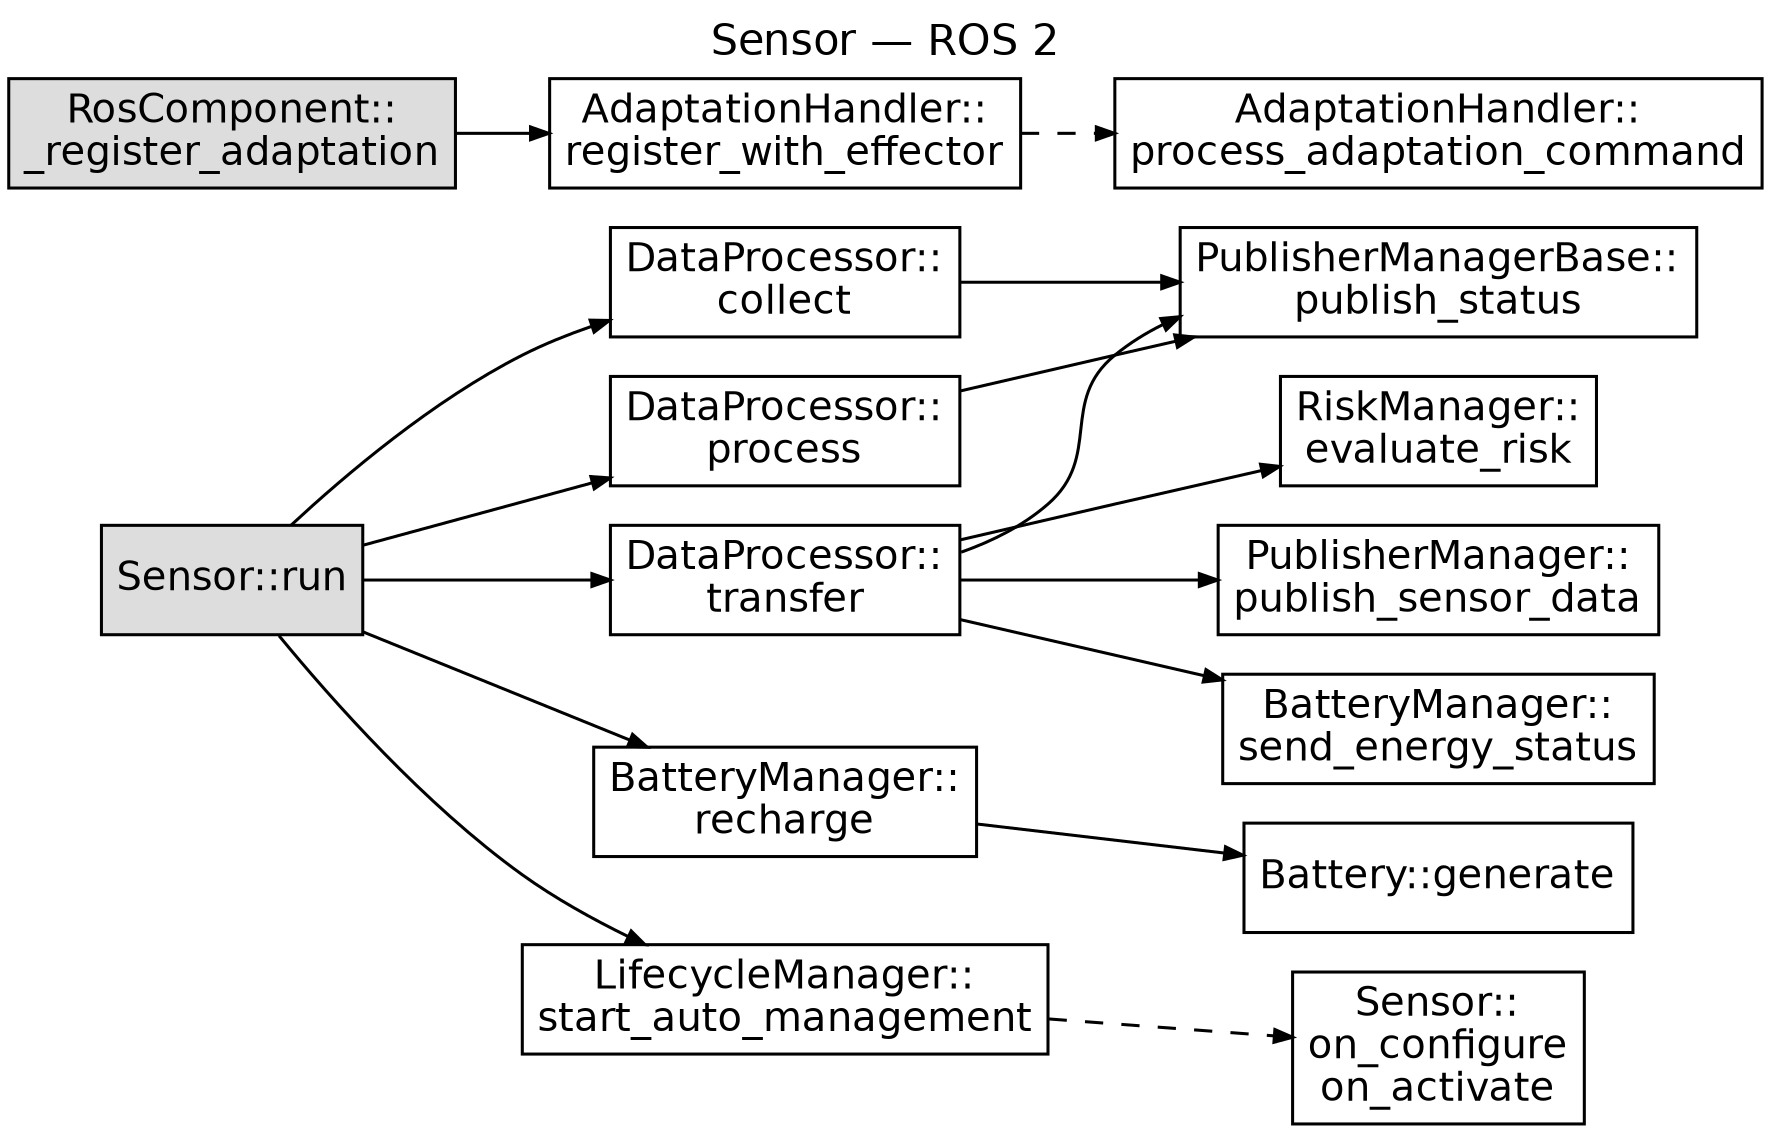
\includegraphics[width=\linewidth]{img/ros2/sensor_tg.png}
\caption{Organização do processamento e das
responsabilidades de \texttt{Sensor} no ROS~2.}
\label{fig:sensorROS2}
\end{figure}

A comunicação com \texttt{CentralHub} também foi reorganizada. No ROS~1, \texttt{CentralHub::run()} estabelece subscrições para os tópicos dos sensores. No ROS~2, \texttt{SensorDataHandler} configura essas subscrições por meio de \texttt{create\_subscription()}, enquanto \texttt{PublisherManager} concentra as operações de publicação. A Figura~\ref{fig:centralHubROS2} apresenta a organização do processamento do \texttt{CentralHub} no ROS~2.

\begin{figure}[htbp]
\centering
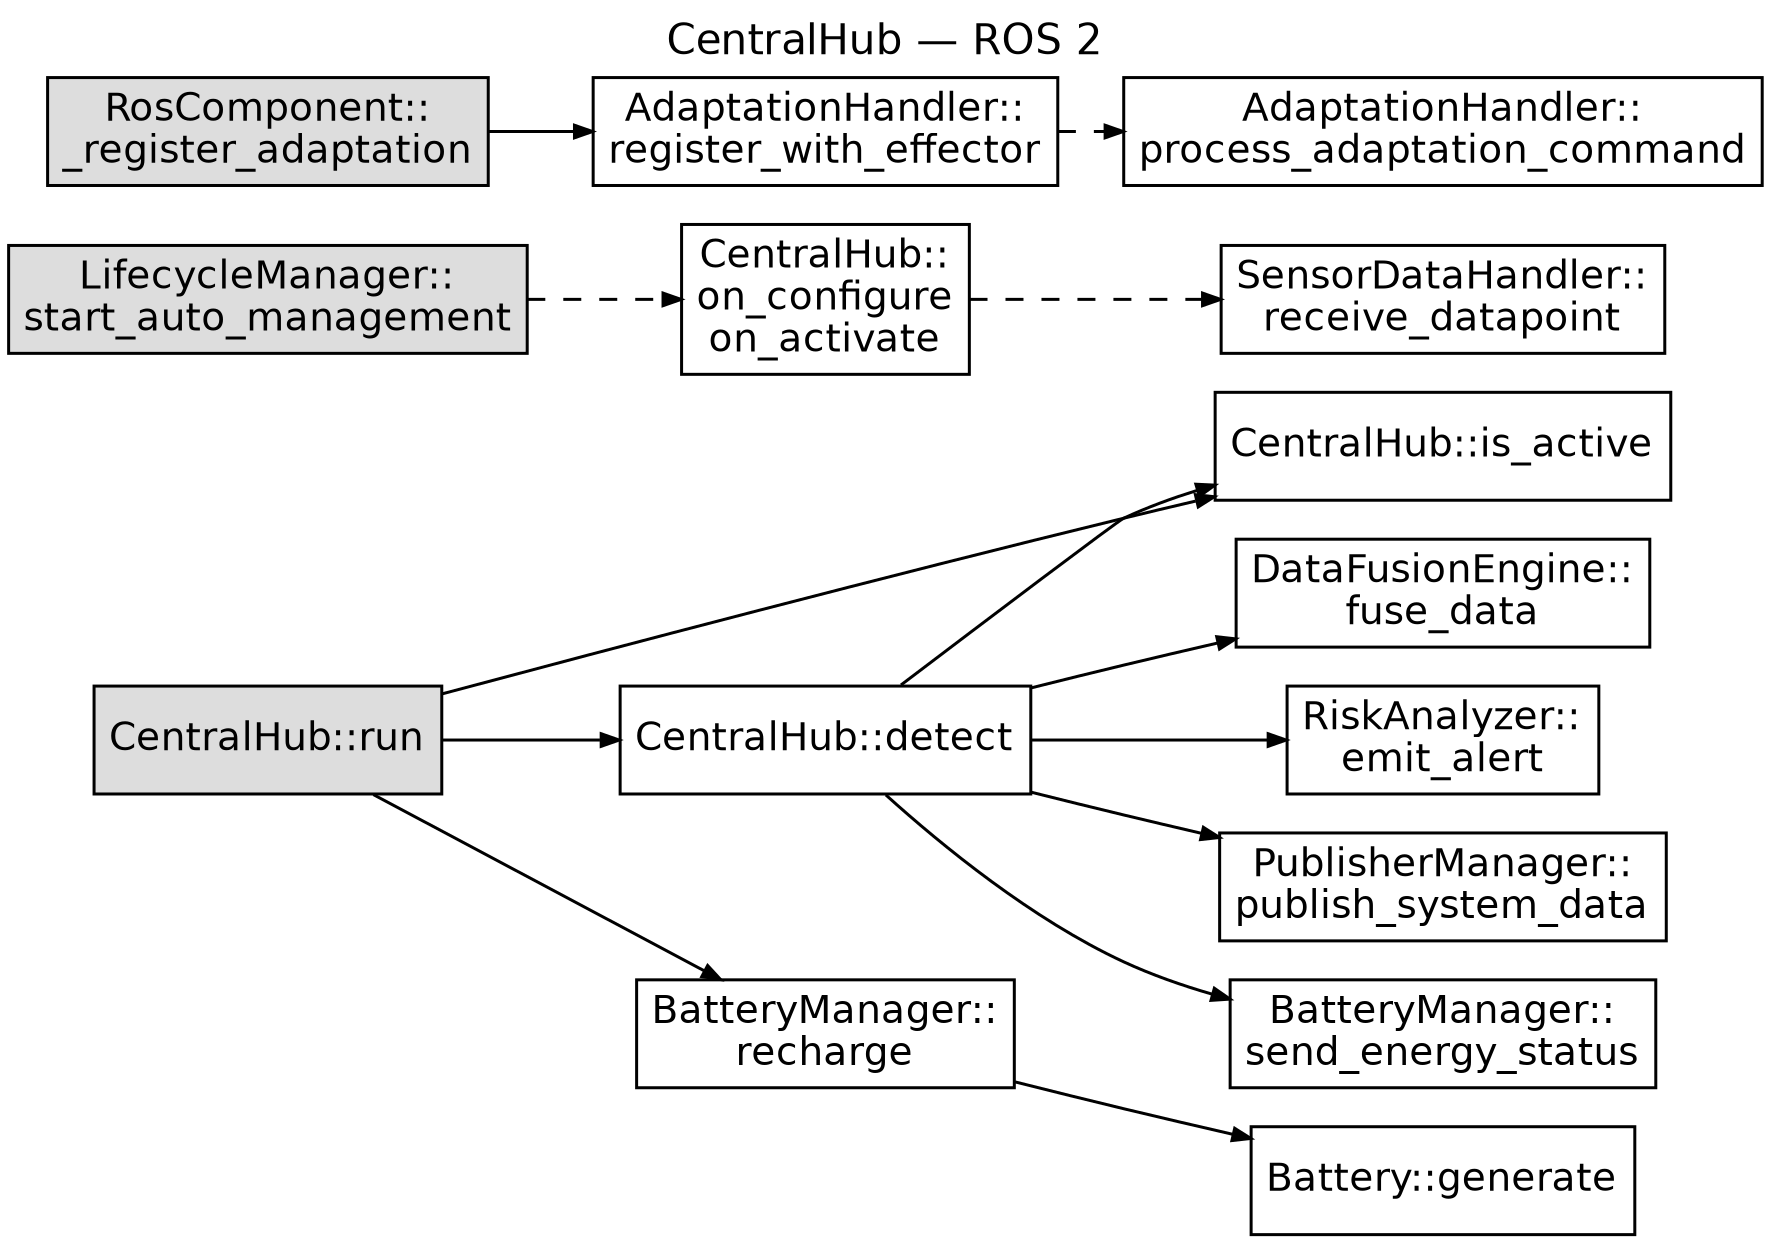
\includegraphics[width=\linewidth]{img/ros2/central_hub_tg.png}
\caption{Organização do processamento e das
responsabilidades de \texttt{CentralHub}
no ROS~2.}
\label{fig:centralHubROS2}
\end{figure}

A avaliação de risco também foi reorganizada. No legado, \texttt{SensorConfiguration} reúne operações de configuração e avaliação por faixas. No ROS~2, essas responsabilidades são distribuídas entre \texttt{RiskManager} e \texttt{RiskEvaluator}. A transformação T3 combina a adaptação das interfaces de comunicação à plataforma ROS~2 com a reorganização interna das responsabilidades de processamento e avaliação de risco.


\subsection{Registro das Transformações de Migração}
\label{subsec:res-planejamento-registro}

A Tabela~\ref{tab:res-migration-record} consolida as transformações identificadas na comparação retrospectiva das implementações. O registro relaciona as responsabilidades do ROS~1, os tratamentos identificados no ROS~2 e os cenários em BDD associados a cada transformação.


\begin{table}[htbp]
\centering
\caption{Registro retrospectivo das transformações de migração da BSN}
\label{tab:res-migration-record}
\scriptsize

\begin{tabularx}{\linewidth}{@{}
p{0.07\linewidth}
p{0.24\linewidth}
p{0.34\linewidth}
X@{}}
\toprule

\textbf{ID} &
\textbf{Responsabilidade no ROS~1} &
\textbf{Transformação identificada no ROS~2} &
\textbf{Contratos BDD associados} \\

\midrule

T1 &
Controle da atividade de \texttt{Sensor} e
\texttt{CentralHub}, considerando o estado
operacional e a bateria. &
Adaptação tecnológica: utilização de
\texttt{RosComponent}, derivada de
\texttt{LifecycleNode}, e de
\texttt{LifecycleManager} para o
gerenciamento do ciclo de vida dos nós. &
BDD05, relacionado à indisponibilidade
do \texttt{CentralHub}; BDD03 e BDD09,
associados a comportamentos que dependem
da operação dos componentes. \\

\addlinespace

T2 &
Coleta e encaminhamento de eventos,
estados e informações de energia por
\texttt{Probe}. &
Ampliação funcional: \texttt{SystemMonitor}
mantém o encaminhamento das informações
e incorpora a supervisão da atividade
dos nós e a detecção da ausência de
\textit{heartbeats}. &
BDD15, relacionado ao encaminhamento
de informações de monitoramento.
A supervisão por \textit{heartbeats}
constitui comportamento adicional
no ROS~2. \\

\addlinespace

T3 &
Coleta, processamento e comunicação
de leituras, além da avaliação
de risco dos sensores. &
Adaptação tecnológica e reorganização
interna: redistribuição das operações
entre \texttt{DataProcessor},
\texttt{SensorDataHandler},
\texttt{PublisherManager},
\texttt{RiskManager} e
\texttt{RiskEvaluator}. &
BDD03, relacionado à transmissão
e recepção de leituras; BDD04,
relacionado à classificação de risco
observável na saída do sistema. \\

\bottomrule
\end{tabularx}
\end{table}



A Tabela~\ref{tab:res-migration-record} constitui o \textit{Migration Transformation Record} reconstruído para a BSN, relacionando as responsabilidades identificadas no ROS~1 às transformações observadas no ROS~2 e aos contratos comportamentais associados.


\section{Estabelecimento da \textit{Ground Truth} e Validação Comportamental da BSN}
\label{sec:resultados-ground-truth-validacao-bsn}
\label{sec:aplicacao-ground-truth-bsn}
\label{sec:resultados-validacao-bsn}

Esta seção reúne os resultados do Estabelecimento da \textit{Ground Truth} Comportamental e da Validação Comportamental. A primeira etapa estabelece uma referência a partir dos critérios BDD, dos testes e das observações do ROS~1 enquanto a segunda confronta essa referência com a implementação migrada em ROS~2
A reconstrução utiliza os resultados os resultados preservados no repositório~\cite{Viana}, os testes do legado e da implementação migrada\footnote{\url{https://github.com/richardjlv/bsn_} e \url{https://github.com/richardjlv/bsn2}.} e os registros de campanhas e testes complementares arquivados em \texttt{bsn\_traces}\footnote{\url{https://github.com/richardjlv/bsn_traces}.}.

\subsection{Preparação dos testes e delimitação dos comportamentos}
\label{subsec:gt-validacao-preparacao}

Os cenários Gherkin recuperados na etapa de Especificação Comportamental foram implementados no legado por definições de passos e mecanismos de observação das interfaces ROS. A infraestrutura histórica empregava \textit{behave} e observação de tópicos pelo ROS CLI mas, posteriormente, parte dos testes ROS~1 foi adaptada para \texttt{pytest-bdd} com \texttt{rostest}. No ROS~2, os passos e a preparação foram adaptados para implementação em Python.

A Tabela~\ref{tab:cenarios-amostra-comportamental} reúne os cenários BDD selecionados para o Estabelecimento da \textit{Ground Truth} Comportamental e a Validação Comportamental, sintetizando condições iniciais, estímulos e resultados esperados dos comportamentos investigados nas duas implementações.

\begin{table}[htbp]
\centering
\caption{Cenários BDD selecionados para a análise
comportamental da BSN}
\label{tab:cenarios-amostra-comportamental}
\footnotesize
\renewcommand{\arraystretch}{1.2}
\begin{tabularx}{\textwidth}{
    @{}
    p{2.45cm}
    X
    X
    X
    @{}
}
\hline
\textbf{Cenário e contrato} &
\textbf{Condição inicial} &
\textbf{Estímulo} &
\textbf{Resultado esperado} \\
\hline

BDD03 / BSN-C01
&
Paciente monitorado por um dos seis sensores.
&
O sensor informa uma nova leitura de sinal vital.
&
O CentralHub recebe a leitura com o valor
informado pelo sensor.
\\

BDD04 / BSN-P09
&
Paciente monitorado pelo oxímetro.
&
O sensor informa uma leitura na faixa
de alto risco.
&
O risco alto é observado na saída
do CentralHub.
\\

BDD06 / BSN-P08
&
Sistema em operação com o mecanismo
de persistência disponível.
&
Um sensor produz uma leitura de
sinal vital.
&
A leitura é persistida e pode ser
recuperada com o valor informado.
\\

BDD07 / BSN-C03
&
O mecanismo de armazenamento apresenta
uma falha.
&
O sistema tenta persistir uma leitura.
&
A falha de persistência é registrada
pelo sistema.
\\

BDD08 / BSN-P10
&
Paciente monitorado pelo termômetro,
com o CentralHub disponível.
&
O termômetro produz leituras que
são processadas pelo sistema.
&
O CentralHub disponibiliza um novo
estado de saúde do paciente.
\\

BDD09 / BSN-C04
&
Paciente monitorado pelo termômetro,
com o CentralHub indisponível.
&
O termômetro continua produzindo
leituras.
&
Não é disponibilizado um novo
estado de saúde pelo CentralHub.
\\

BDD20 / BSN-C11
&
Confiabilidade do sensor acima do
limiar de adaptação.
&
O sistema é observado durante essa
condição de confiabilidade.
&
Não são emitidos comandos de
adaptação da frequência.
\\

\hline
\end{tabularx}

\vspace{0.2cm}
\begin{minipage}{\textwidth}
\footnotesize
\textbf{Fonte:} Elaboração própria com base nos
cenários BDD da BSN e na rastreabilidade
no repositório~\cite{Viana}.
\end{minipage}
\end{table}

Como exemplo da construção da referência no ROS~1, o cenário BDD03, apresentado na Listagem~\ref{lst:bsn-c01-ros1}, foi relacionado ao arquivo \texttt{check\_bsn.feature} e às definições de passos em \texttt{test\_check\_bsn.py}. A verificação compara valores capturados nos tópicos do sensor e do CentralHub por meio de \path{count_and_get_matching_elements_with_time}. A Figura~\ref{fig:gt-instrumentacao-bdd03} sintetiza os artefatos identificados na inspeção.

\begin{figure}[h]
\centering
\begin{tikzpicture}[
  >=Stealth,
  node distance=4mm,
  artefato/.style={draw,rounded corners,align=center,
    text width=0.82\linewidth,minimum height=8mm,font=\small,inner sep=3pt}
]
\node[artefato] (gherkin) {\texttt{check\_bsn.feature}: cenário BDD03};
\node[artefato,below=of gherkin] (steps) {\texttt{test\_check\_bsn.py}: definições
de passos};
\node[artefato,below=of steps] (capture) {\texttt{conftest.py}: preparação e captura
compartilhadas};
\node[artefato,below=of capture] (oracle) {\texttt{test\_check\_bsn.py}: comparação
de valores e asserção};
\node[artefato,below=of oracle] (result) {Relatório de execução JUnit/XML};
\draw[->] (gherkin) -- (steps);
\draw[->] (steps) -- (capture);
\draw[->] (capture) -- (oracle);
\draw[->] (oracle) -- (result);
\end{tikzpicture}
\caption{Instrumentação de BDD03 no ROS~1 reconstruída a partir dos
artefatos de teste.}
\label{fig:gt-instrumentacao-bdd03}
\end{figure}
\FloatBarrier

\subsection{Interpretação dos oráculos e correspondência entre as versões}
\label{subsec:gt-validacao-oraculos}

A \textit{Ground Truth} comportamental do ROS~1 foi examinada relacionando os critérios de aceitação às asserções efetivamente implementadas. Em seguida, foram identificadas as verificações correspondentes no ROS~2, considerando as adaptações das interfaces, da preparação e dos mecanismos de observação. A Tabela~\ref{tab:gt-validacao-oraculos} apresenta os mesmos grupos de cenários nas duas etapas.

\begin{table}[htbp]
\centering
\footnotesize
\caption{Comparação dos oráculos da amostra no ROS~1 e no ROS~2}
\label{tab:gt-validacao-oraculos}
\begin{tabularx}{\textwidth}{@{}p{0.18\textwidth}XX@{}}
\toprule
\textbf{Cenário} & \textbf{Oráculo observado no ROS~1} &
\textbf{Correspondência e limite no ROS~2} \\
\midrule
BDD03 / BSN-C01 &
Busca valores coincidentes nas capturas dos tópicos do sensor e do CentralHub. &
Mantém a comparação de valores com interfaces ros de captura adaptadas.
\\
\addlinespace
BDD04 / BSN-P09 &
Busca correspondência de riscos e presença de classificação alta, na faixa de
66 a 100, na saída observada. &
Verifica risco alto nas interfaces correspondentes. A aprovação não demonstra
que o CentralHub tenha calculado a classificação nem a equivalência integral
do processamento. \\
\addlinespace
BDD06--BDD07 / BSN-P08 &
O cenário positivo observa uma mensagem \texttt{Status} em \texttt{/persist};
o negativo é marcado como falha esperada. &
A verificação positiva acompanha a atividade do sensor e registros filtrados
pela origem; o caso negativo também é marcado como falha esperada.
Nenhuma das asserções recupera a leitura fisiológica armazenada. \\
\addlinespace
BDD08--BDD09 / BSN-P10 &
Verifica a presença de leituras válidas do termômetro e de valores distintos de patient\_status entre 0 e 100 no cenário positivo. No negativo, exige leituras do termômetro sem publicação de estado de saúde a partir do CentralHub. &
No ROS 2, são aplicados os mesmos critérios de aceitação do ROS 1 após a revisão de 26/10/2026. As aprovações demonstram a observação dos comportamentos esperados. \\
\addlinespace
BDD20 / BSN-C11 &
Exige ausência de comandos de adaptação sob confiabilidade estável;
resultado marcado como \texttt{XFAIL}. &
O comportamento correspondente também foi investigado na adaptação ROS~2,
com \texttt{XFAIL}. Os testes BDD não estabelecem, isoladamente, igualdade
dos estados de confiabilidade nas execuções. \\
\bottomrule
\end{tabularx}
\par\smallskip
{\footnotesize\textbf{Fonte:} elaboração própria a partir da inspeção dos
testes e da análise de oráculos~\cite{Viana}.}
\end{table}
\FloatBarrier

A comparação evidencia que a correspondência entre cenários das duas implementações não implica equivalência do alcance de seus oráculos. A interpretação das aprovações depende das propriedades efetivamente verificadas pelas asserções, dos estímulos e das condições de observação.


\subsection{Confronto das evidências de execução}
\label{subsec:gt-validacao-execucoes}

Os resultados de execução dos cenários selecionados foram confrontados nas duas implementações com base nas campanhas e reexecuções documentadas no repositório~\cite{Viana}. A Tabela~\ref{tab:gt-validacao-campanhas} apresenta os resultados gerais, distinguindo as campanhas completas das revalidações parciais, enquanto a Tabela~\ref{tab:gt-validacao-amostra} detalha os casos da amostra.

\begin{table}[htbp]
\centering
\small
\caption{Campanhas BDD utilizadas como evidência histórica}
\label{tab:gt-validacao-campanhas}
\begin{tabularx}{\textwidth}{@{}Xrrrr@{}}
\toprule
\textbf{Plataforma e recorte} & \textbf{Casos} & \textbf{PASS} &
\textbf{XFAIL} & \textbf{FAIL} \\
\midrule
ROS~1, oito famílias isoladas (26/10/2026) & 51 & 49 & 2 & 0 \\
ROS~2, oito famílias isoladas (25/10/2026) & 51 & 38 & 10 & 3 \\
ROS~2, revalidação selecionada (02/11/2026) & 11 & 10 & 1 & 0 \\
\bottomrule
\end{tabularx}
\par\smallskip
{\footnotesize\textbf{Fonte:}  relatórios internos
JUnit/XML preservados em \texttt{bsn\_traces}~\cite{Viana}. A última linha não deve ser
somada às anteriores; resultados de executores externos do \texttt{rostest}
não foram contabilizados como novos casos.}
\end{table}
\FloatBarrier

O confronto da Tabela~\ref{tab:gt-validacao-amostra} inclui as reexecuções específicas de estado de saúde com critérios comuns de 26/10/2026, considerando as datas e condições de cada execução separadamente.

\begin{table}[htbp]
\centering
\footnotesize
\caption{Confronto retrospectivo dos mesmos cenários no ROS~1 e no ROS~2}
\label{tab:gt-validacao-amostra}
\begin{tabularx}{\textwidth}{@{}p{0.18\textwidth}XX@{}}
\toprule
\textbf{Cenário} & \textbf{Evidência ROS~1} & \textbf{Evidência ROS~2} \\
\midrule
BDD03 / BSN-C01 &
A campanha ROS~1 de 26/10 registrou aprovação dos casos de recepção da
família \texttt{check\_bsn}. & Na coleta ROS~2 de 25/10, o caso
do oxímetro falhou por ausência de dados capturados. Na revalidação
de 02/11, a família \texttt{check\_bsn} registrou oito aprovações. \\

\addlinespace
BDD04 / BSN-P09 &
Caso de risco alto com \texttt{PASS} em \texttt{check\_bsn} (26/10). &
\texttt{PASS} no caso correspondente em 25/10 e na revalidação de 02/11. \\
\addlinespace
BDD06--BDD07 / BSN-P08 &
Um \texttt{PASS} nominal e um \texttt{XFAIL} de falha de armazenamento
(26/10). &
Falha nominal e \texttt{XFAIL} em 25/10; em 02/11,
um \texttt{PASS} e um \texttt{XFAIL}. A falha esperada ocorreu em
etapa de preparação na coleta ROS~2 de 25/10. \\
\addlinespace
BDD08--BDD09 / BSN-P10 &
Dois \texttt{PASS} em execução posterior com oráculo comum (26/10). &
Dois \texttt{PASS} com os mesmos critérios de asserção na execução de
26/10; isso não iguala os estímulos nem as sequências observadas. \\
\addlinespace
BDD20 / BSN-C11 &
\texttt{XFAIL} no critério de ausência de comandos (26/10). &
\texttt{XFAIL} no critério correspondente na campanha de adaptação
(25/10); requer interpretação dos estados operacionais e dos estímulos. \\
\bottomrule
\end{tabularx}
\par\smallskip
{\footnotesize\textbf{Fonte:} elaboração própria a partir dos
resultados por caso, rastros e revalidações no repositório ~\cite{Viana} \texttt{bsn\_traces}.}
\end{table}
\FloatBarrier

Em BDD06--BDD07, o resultado \texttt{XFAIL} não fornece o mesmo tipo de evidência nas duas plataformas: no legado, a falha esperada foi registrada no passo de verificação, enquanto na coleta ROS~2 de 25/10 ocorreu durante a preparação da falha simulada. Assim, as duas marcações não confirmam a ocorrência de um mesmo defeito de armazenamento.

As execuções com oráculo comum de estado de saúde estão identificadas, respectivamente, como \path{ros1_20261026T222148Z\_health_status_t2w8_ul0} e \path{ros2_20261026T221156Z\_uowmc6al} no repositório~\cite{Viana}. A identificação das campanhas é necessária porque os relatórios mais antigos de \texttt{health\_status} utilizavam critérios diferentes.


\subsection{Evidências Complementares aos Testes BDD}
\label{subsec:gt-validacao-complementar}

Além das campanhas BDD, o repositório~\cite{Viana} documenta testes complementares que permitem aprofundar a verificação de comportamentos selecionados. Esses testes utilizam entradas controladas ou testes direcionados a responsabilidades específicas, complementando as observações dos cenários BDD sem constituir novas execuções desses mesmos cenários.

Como verificação complementar do processamento do CentralHub, um testes utilizou mensagens sintéticas com riscos e identificadores conhecidos. Nas duas implementações, foram aprovadas nove fases de verificação, com a sequência esperada de estados de saúde 20, 90 e 20, repetida três vezes. Diferentemente de BDD03, esse testes verifica as respostas do CentralHub a mensagens diretamente injetadas, sem exercitar a aquisição original das leituras pelos sensores.

Na classificação de risco (BDD04), quatro casos foram executados diretamente nas classes responsáveis pela classificação nas implementações C++ e Python, obtendo aprovação em ambas. O defeito B7, documentado no repositório, consistia na utilização incorreta dos intervalos fisiológicos para determinar a categoria de risco, em vez das faixas percentuais correspondentes. Os mesmos casos reprovaram quando esse defeito foi reintroduzido em uma cópia da classe C++. Esse resultado demonstra a capacidade dos testes complementares de detectar o defeito investigado, ampliando a verificação da classificação para além da observação de risco alto realizada pelo cenário BDD04.

Quanto à persistência (BDD06), um testes controlado verificou a gravação e a recuperação de 30 registros no tópico \texttt{Status} em cada implementação, inclusive após o encerramento dos processos. Esse resultado complementa o BDD06, cuja asserção observa o encaminhamento dos registros.



Por fim, na adaptação (BDD20), no repositório foi~\cite{Viana} documentado testes controlados com valores de confiabilidade fornecidos aos controladores das duas implementações. Inicialmente, foram identificadas diferenças nas condições de erro nulo e de erro dentro da margem de adaptação. Após uma correção no controlador ROS~1, os quatro casos controlados foram aprovados nas duas versões, incluindo a ausência de comandos nessas condições.

Esse resultado sustenta a correspondência das decisões dos controladores para os valores ensaiados, mas não comprova a recuperação da malha completa nem a alteração efetiva da frequência dos sensores.



\subsection{Síntese da referência e do alcance da validação}
\label{subsec:gt-validacao-sintese}

O Estabelecimento da \textit{Ground Truth} Comportamental resultou em uma referência delimitada pelos cenários BDD, pelas asserções e pelos resultados de execução no ROS~1. O confronto com o ROS~2 permitiu identificar correspondências para os critérios efetivamente verificados, além de discrepâncias e limitações dos oráculos e das condições de execução, especialmente na persistência e na adaptação. Os testes complementares ampliaram a investigação de responsabilidades específicas.


